\documentclass[tikz,border=2pt]{standalone}
\usepackage{amsmath}
\usepackage{pgfplots}
\pgfplotsset{compat=1.18}

\begin{document}
% f(x)=e^x-1 and g(x)=sin 2x both vanish at 0; near 0 each looks like its tangent line, so the
% ratio f/g behaves like the ratio of the slopes f'(0)/g'(0) = 1/2.
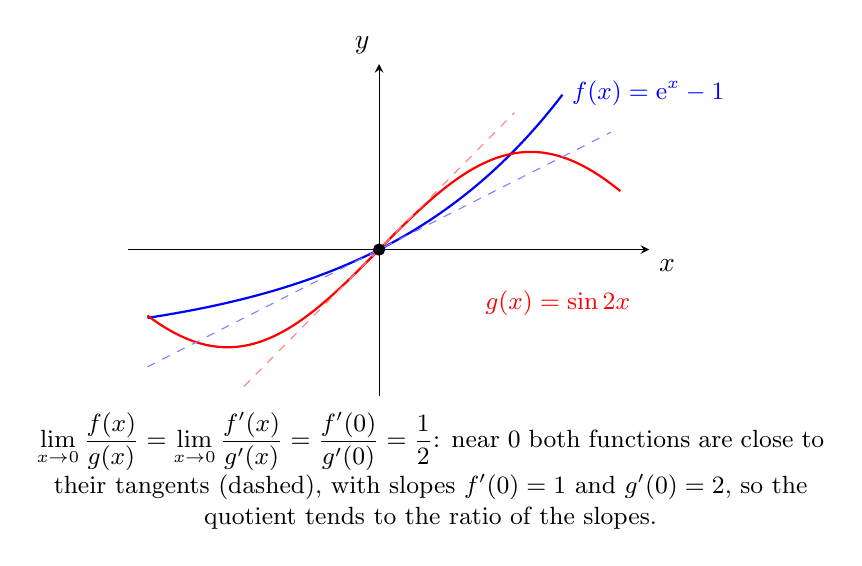
\begin{tikzpicture}
	\begin{axis}[
		axis lines=middle,
		xmin=-1.3, xmax=1.4,
		ymin=-1.5, ymax=1.9,
		xtick=\empty, ytick=\empty,
		xlabel={$x$}, ylabel={$y$},
		xlabel style={below right}, ylabel style={above left},
		samples=160, smooth, clip=false,
		width=8.2cm, height=5.8cm
		]
		\addplot[thick, blue, domain=-1.2:0.95] {exp(x)-1};
		\addplot[thick, red, domain=-1.2:1.25] {sin(deg(2*x))};
		\addplot[blue!50, dashed, domain=-1.2:1.2] {x};
		\addplot[red!50, dashed, domain=-0.7:0.7] {2*x};
		\addplot[only marks, mark=*, black] coordinates {(0,0)};
		\node[blue, anchor=west, font=\small] at (axis cs:0.95,1.6) {$f(x)=\mathrm{e}^x-1$};
		\node[red, anchor=west, font=\small] at (axis cs:0.5,-0.55) {$g(x)=\sin 2x$};
	\end{axis}
	\node[anchor=north, align=flush center, text width=10cm, font=\small] at ([yshift=-2pt]current axis.outer south) {$\displaystyle\lim_{x\to0}\frac{f(x)}{g(x)}=\lim_{x\to0}\frac{f'(x)}{g'(x)}=\frac{f'(0)}{g'(0)}=\frac12$: near $0$ both functions are close to their tangents (dashed), with slopes $f'(0)=1$ and $g'(0)=2$, so the quotient tends to the ratio of the slopes.};
\end{tikzpicture}
\end{document}
